\notechapter{N-20260408}{Volumes, Spatial Regions, and Order of Integration}


\section{Volume by double and triple integrals}

If a curved cylinder has top $z=f(x,y)$ over a plane region $D$, then its volume is
\[
  V=\iint_D f(x,y)\,dx\,dy.
\]
For a solid region $\Omega$,
\[
  V=\iiint_\Omega 1\,dV.
\]
These formulas are the same idea: integrate a density of $1$ over the appropriate measure.

\section{Describing spatial regions}

A region may be $xy$-simple, $yz$-simple, or $zx$-simple.  For example,
\[
  \Omega=\{(x,y,z):(x,y)\in D,\ z_1(x,y)\le z\le z_2(x,y)\}.
\]
If a single description is impossible, split the region.  Most difficult triple-integral problems are difficult because of the geometry of $\Omega$, not because of the antiderivatives.

\begin{figure}[H]
\centering
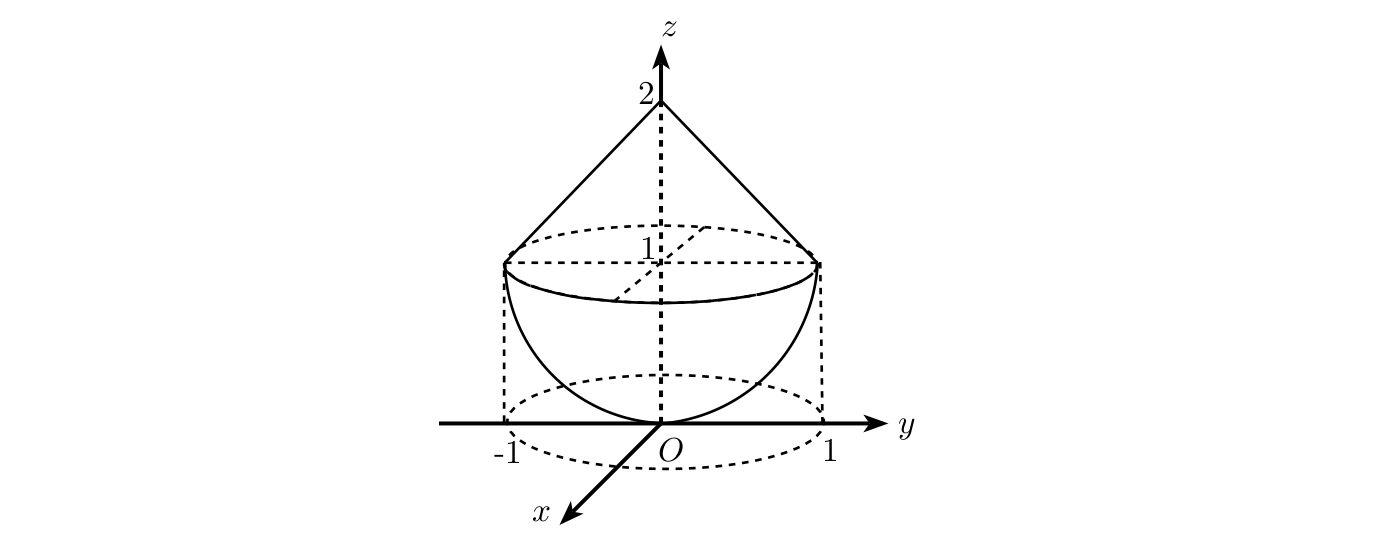
\includegraphics[width=0.78\textwidth,height=0.74\textheight,keepaspectratio]{figures/notes-md/N-20260408/N-20260408-fig-01-composite-solid-hemisphere-and-cone.png}
\caption{A composite solid with a hemispherical part and a conical part.  The picture is used to decide cross-sections and height bounds before writing the integral.}
\end{figure}


\section{Changing order of integration}

Changing the order means projecting the region onto a different coordinate plane and rewriting the boundary.  The safe procedure is: identify the shadow, determine the inner variable's lower and upper surfaces, and split the shadow if necessary.




\begin{figure}[H]
\centering
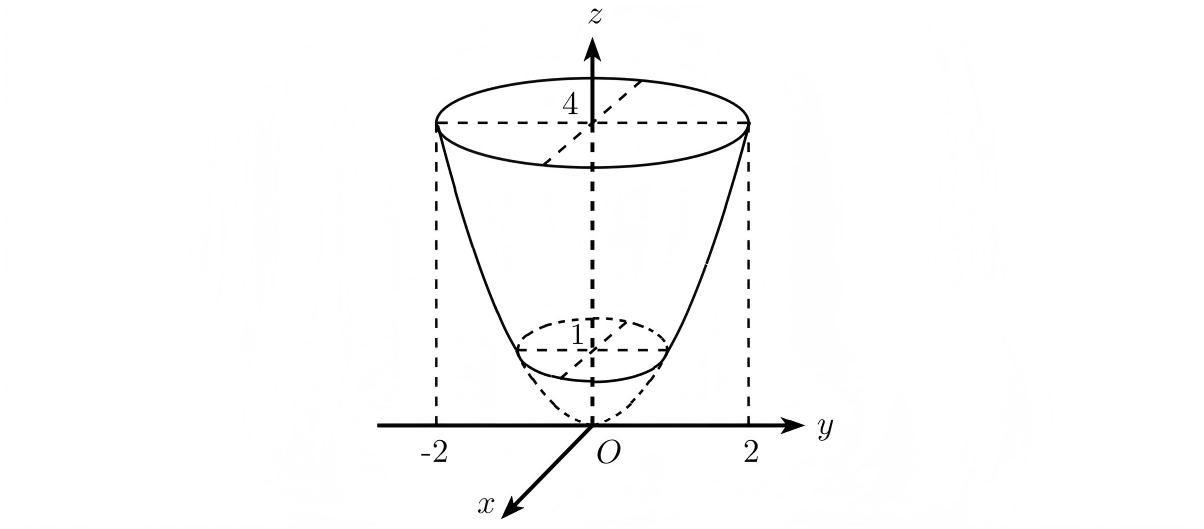
\includegraphics[width=0.78\textwidth,height=0.74\textheight,keepaspectratio]{figures/notes-md/N-20260408/N-20260408-fig-02-truncated-rotational-solid.png}
\caption{A rotational solid with circular cross-sections at different heights.  Such diagrams are read by projecting to the base plane and then recovering the vertical bounds.}
\end{figure}

\section{Expanded synthesis and advanced context}

Integration over regions is geometric bookkeeping.  The same solid can be sliced in many directions, and the best order is the one that makes both the limits and the integrand transparent.



\paragraph{Expanded synthesis.}
For this chapter, the elementary material should be read as a study of what remains invariant when coordinates change. The earlier sections (`Volume by double and triple integrals`, `Describing spatial regions`, `Changing order of integration`, `Higher viewpoint`) compute with arrays, bases, pivots, determinants, or eigenvectors; the deeper object is a linear map together with the spaces it acts on. A matrix is a representation of that map after bases have been chosen. This is why formulas such as
\[
  A' = P^{-1}AP,\qquad \widetilde A = T^{-1}AS
\]
are not cosmetic: they distinguish an intrinsic morphism from a coordinate description.

The structural hierarchy is as follows. Kernels record what a map forgets, images record what it reaches, cokernels record obstructions to solvability, and quotients record information after an equivalence has been imposed. Determinants act on the top exterior power and therefore measure oriented volume; traces are invariant under cyclic rearrangement and become characters in representation theory; adjoints depend on an inner product and lead to self-adjoint spectral theory.

A useful way to return to the computations is to ask, for every formula, which invariant it is measuring. Row reduction measures rank and kernel; diagonalization measures decomposition into invariant subspaces; Gram--Schmidt measures orthogonal projection; positive definiteness measures ellipsoid geometry; tensor notation measures how components transform. The elementary methods are therefore the finite-dimensional laboratory in which duality, quotienting, functoriality, and spectral decomposition can be seen clearly.


\section{Expanded region reconstruction}

Spatial-integration examples usually fail at the same point: the student sees the integral but not the solid.  A good reconstruction process is:

\begin{enumerate}[(i)]
  \item identify the surfaces that bound the solid;
  \item draw or mentally project the solid onto a coordinate plane;
  \item decide which variable has the simplest lower and upper bounds;
  \item split the region only when a single set of bounds would hide a boundary change.
\end{enumerate}

For a solid between $z=z_1(x,y)$ and $z=z_2(x,y)$ above $D$, the volume is
\[
  V=\iint_D [z_2(x,y)-z_1(x,y)]\,dA.
\]
This is the double-integral version of ``top minus bottom.''

\section{Why pictures remain useful}
